\paragraph{Completed follow-up evidence.}
The completed PubMed/SAGE two-rate cohort gives STRATA test accuracy 0.71623, versus 0.67902 for Single-Grassmann and 0.69061 for AdamW: descriptive gains of 3.721 and 2.562 percentage points. Each method selects its rate using terminal-100 validation accuracy. Its archived optimizer tensor state, including fixed probes, is 58.1\% of AdamW's. Table~\ref{tab:pubmed-resources} gives all five methods, including stronger competitors; this is a comparison-specific benefit, not a graph-family or significance claim.
\begin{table*}[t]\centering\footnotesize
\caption{PubMed/SAGE: validation-selected two-rate, seed-42, 1000-epoch comparisons. State is unique optimizer tensor storage read from the final checkpoint, including probes. Peak is maximum recorded CUDA allocation; wall time is shared-server epoch timing, not isolated throughput.}\label{tab:pubmed-resources}
\begin{adjustbox}{max width=\linewidth}
\begin{tabular}{lrrrrr}\toprule Method & Val acc & Test acc & State MiB & Peak MiB & ms/epoch\\\midrule
\rowcolor{oursbg}
STRATA & 0.7179 & 0.7162 & 2.32 & 391.1 & 29.6 \\
Single-G & 0.7067 & 0.6790 & 1.82 & 390.6 & 24.2 \\
AdamW & 0.7041 & 0.6906 & 3.99 & 392.7 & \textbf{16.6} \\
GaLore & \textbf{0.7590} & \textbf{0.7580} & \textbf{1.26} & \textbf{390.0} & 22.3 \\
Independent & 0.7419 & 0.7415 & 2.20 & 391.0 & 27.3 \\
\bottomrule\end{tabular}
\end{adjustbox}\end{table*}
\begin{figure*}[t]\centering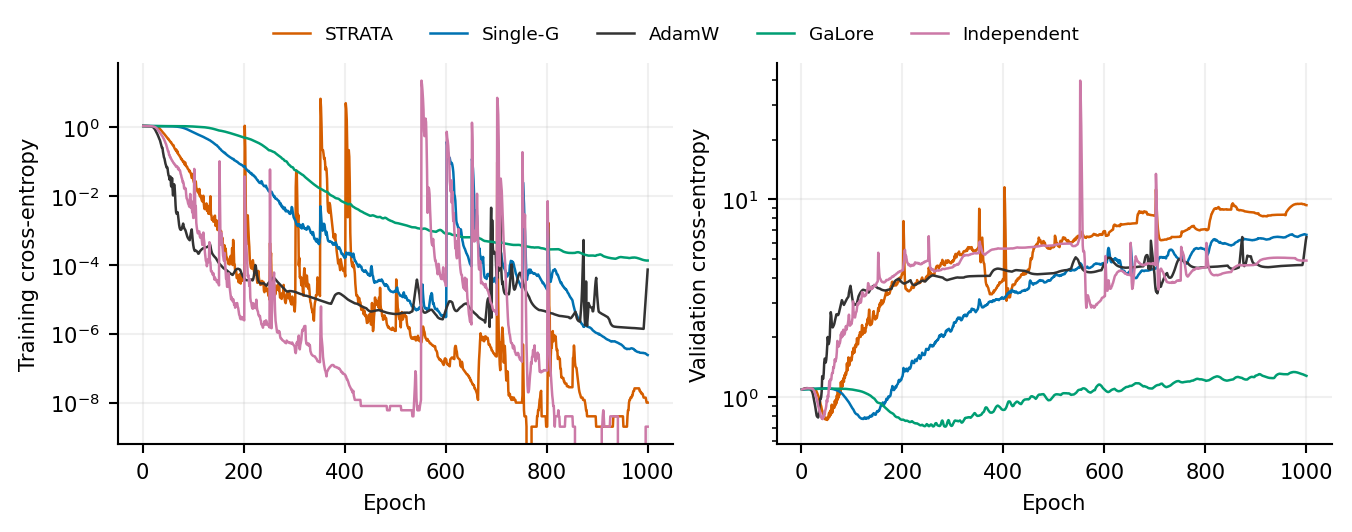
\includegraphics[width=.98\linewidth]{figures/fig_evidence_pubmed.png}\caption{Completed PubMed/SAGE training and validation trajectories. Each of five methods selects its learning rate using terminal-100 validation accuracy after both full-budget candidates finish. All trajectories are raw; held-out test outcomes are reported in Table~\ref{tab:pubmed-resources}.}\label{fig:pubmed-positive}\end{figure*}
The completed default-protocol PubMed architectures are gat, gcn, gcnii, sage; positive STRATA--Single-G test differences occur in gcn, sage. Every completed architecture remains in Table~\ref{tab:new-cohorts}. Further controlled ablations and an equal-budget flag-step sweep are reported in Appendix~\ref{app:evidence-extension}; experimental variants do not overwrite default-protocol results.
\paragraph{Mechanism evidence in the positive setting.} Both rates for all ten PubMed/SAGE interventions are complete (22 configurations including the full controls). Full STRATA reaches 71.623\%, exceeding every validation-selected ablation by 0.435--3.984 percentage points (Table~\ref{tab:pubmed-ablations}). This supports the combined configuration in this setting; interventions that also alter resets or the covariance objective do not isolate a single geometric cause.
\paragraph{Matched flag-step search.} In the completed exploratory six-candidate grid for each geometric method, validation selects STRATA at $\xi=10$ and $\eta=10^{-3}$, with test accuracy 73.383\%, versus 67.902\% for Single-Grassmann and 74.151\% for Independent. The STRATA--Single-G difference is 5.481 percentage points; STRATA improves by 1.760 points over its default-step result. Table~\ref{tab:xi-sweep} and the full profiles retain every setting. This is a separate sensitivity result, and Independent remains stronger on held-out test accuracy.
\paragraph{Equal-state follow-up.} A resource-only calibration selects Single-Grassmann rank 82, whose stored optimizer tensor state differs from STRATA R64 by -0.408\%. After the same six-candidate validation search for both methods, test accuracies are 73.383\% and 72.923\%, respectively (signed STRATA difference +0.460 percentage points; Table~\ref{tab:memory-control}). At the default flag step, the two-rate validation selections instead give STRATA 71.623\% and Single-G R82 72.923\%. Thus extra state is a material confound in the equal-rank comparison, and the retained six-grid gain is smaller and protocol-dependent.
